%%%%%%%%%%%%%%%%%%%%%%%%%%%%%%%%%%%%%%%%%%%%%%%%%%%%%%%%%%%%%%%%%%%%%%%%%%%%%%%
% Chapter 2: Título del capítulo 2
%%%%%%%%%%%%%%%%%%%%%%%%%%%%%%%%%%%%%%%%%%%%%%%%%%%%%%%%%%%%%%%%%%%%%%%%%%%%%%%

%++++++++++++++++++++++++++++++++++++++++++++++++++++++++++++++++++++++++++++++

%++++++++++++++++++++++++++++++++++++++++++++++++++++++++++++++++++++++++++++++
\section{Optimización Global}
\label{sec:OPT}
%%%%%%%%%%%%%%%%%%%%%%%%%%%%%%%%%%%%%%%%%%%%%%%%%%%%%%%%%%%%%%%%%%%%%%%%%%%%%%


La Optimización Global trata de optimizar una función o un conjuntos de funciones dentro de un intervalo especificado y teniendo en cuenta diversos criterios y/o restricciones. Por lo general, el objetivo de la optimización global es la de minimizar ese conjunto de funciones nombrado aunque también se puede tratar el caso de la búsqueda del óptimo global. 
La optimización global se basa en encontrar aquel valor mínimo o máximo global dentro del espacio de búsqueda de la función \textbf{\textit{f}} a optimizar. La elección de la técnica empleada para encontrar el óptimo global resulta resulta de gran importancia dado que la función \textbf{\textit{f}} puede tener muchos óptimos locales que pueden llevar al algoritmo a una \textbf{convergencia prematura} y evitar que el algoritmo escape de un óptimo local. \\
El objetivo de la optimización global, considerando un problema de minimización, es encontrar un vector $X* \in \Omega$ tal que $f(X*) \leq f(X)$ para todo $X \in \Omega$. \cite{Segredo2017}.
En este caso particular, tratamos la optimización de tipo \textbf{\textit{box-constrained}}, donde la región factible $\Omega$ está definida por un límite inferior ($a_{i}$) y superior ($b_{i}$) para cada una de las variables de la función, por ejemplo: $\Omega = \prod^{D}_{i=1}[a_{i}, b{i}]$. \cite{Segredo2017}


%%%%%%%%%%%%%%%%%%%%%%%%%%%%%%%%%%%%%%%%%%%%%%%%%%%%%%%%%%%%%%%%%%%%%%%%%%%%%%
\section{Técnicas meta-heurísticas}
\label{sec:META}
%%%%%%%%%%%%%%%%%%%%%%%%%%%%%%%%%%%%%%%%%%%%%%%%%%%%%%%%%%%%%%%%%%%%%%%%%%%%%%

Las meta-heurísticas son un sub-conjunto de métodos de optimización que se encuentran incluidas dentro del conjunto de métodos heurísticos que a su vez forman parte de los métodos aproximados.

\begin{figure}
  \caption{Métodos de optimización.}
  \centering
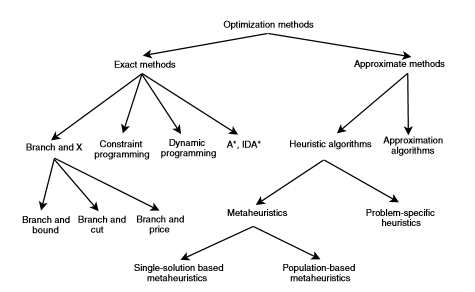
\includegraphics[scale=1.0]{images/meta}\\[10mm]
\end{figure}

A diferencia de los métodos de optimización exactos, las meta-heurísticas nos permiten obtener soluciones factibles a problemas complejos en un tiempo aceptable, aunque no nos garantizan obtener la solución óptima global.\cite{metaheuristics} En los últimos años estás técnicas algorítmicas han ganado una gran popularidad dado que han demostrado su efectividad y eficiencia en muchos campos y con una gran cantidad de problemas distintos.

En cuanto a las distintas meta-heurísticas podemos encontrar hoy en día, podemos diferenciar las siguientes categorías\cite{metaheuristics}:

\begin{itemize}
    \item Búsquedas Locales: Greedy Randomized Adaptive Search Procedure (GRASP) \cite{GRASP}
    \item Heurísticas Voraces: Simulated Annealing (SA) \cite{SA}
    \item Estrategías Evolutivas: Covariance Matrix Adaptation Evolutionary Strategy (CMA-ES)\cite{CMA}, Differential Evolution (DE) \cite{DE1, DE2, DE3}
    \item Algoritmos Genéticos: Coevolutionary algorithms (CEA) \cite{COE1, COE2, COE3}
\end{itemize}


Esta gran variedad de meta-heurísticas se debe principalmente al gran abanico de criterios que podemos definir a la hora de diseñar una meta-heurística. Generalmente, las meta-heurísticas, y en especial, los algoritmos evolutivos, buscan un balance entre ambas propiedades (intensificación/diversificación), aunque es cierto, que algunas, como la búsqueda local, se centran principalmente en intensificar.. Las técnicas de intensificación son aquellas que priorizan una solución prometedora explorándola antes que las soluciones menos prometedores. Por el contrario, las técnicas de diversificación se aseguran que en las regiones menos prometedoras son visitadas para evitar los óptimos locales.
En segundo lugar, debemos tener en cuenta los siguientes criterios:

\begin{itemize}
    \item Métodos inspirados en la naturaleza: Es común inspirarse en el compartimiento de animales o bien de procesos físicos para diseñar un método meta-heurístico que emule ese comportamiento. Por ejemplo: Ant Bee Colonies o Simulated Annealing.
    \item Determinísticos o Estocásticos: Podemos optar por tomar decisiones deterministas o emplear reglas aleatorias durante la búsqueda de nuevas soluciones.
    \item Métodos basados en poblaciones o basados en una única solución: Por un lado nos podemos basar en un conjunto de soluciones factibles que combinaremos entre ellas aplicando diversos operadores para obtener un  nuevo conjunto de soluciones \textit{"hijas"} potencialmente mejores. O bien, podemos optar por utilizar una única solución al problema que transformaremos en cada iteración del algoritmo.
    \item Iterativos o voraces: En este aspecto podemos contemplar comenzar con un conjunto de soluciones al problema e ir transformando dichas soluciones en cada iteración del algoritmo para obtener nuevas soluciones. Al contrario, en una estrategia voraz (Greedy) comenzamos sin una solución factible al problema y en cada iteración incluiremos una variable de decisión hasta obtener la solución completa.
\end{itemize}

\subsection{Representación}

En las técnicas algorítmicas en general nos podemos encontrar con diversas maneras de representar la solución al problema y en las meta-heurísticas estás son las comunes\cite{metaheuristics}:

\bigskip

\begin{itemize}
    \item Cadena binaria: Utilizada en problemas de decisiones 
    \item Vector de valores naturales: Problemas de asignación
    \item Vector de números reales: Utilizada en problemas de optimización continua y/o optimización global.
    \item Secuencia: Empleada en problemas de rutas y de planificación de tareas.
\end{itemize}

Dadas las características del concurso seleccionado para este Trabajo de Fin de Grado, la representación empleada fue \textbf{Vector de valores reales} dado que cada elemento del vector denota un valor dentro del dominio de la función para cada una de las \textbf{\textit{n variables}} que posee.
